%! TEX root = ../../main.tex

\subsection{Versioning}%
\label{sub:Versioning}
The topic of versioning does not only come up in the context of microservices.
In traditional software releases, e.g.\ of \textit{Microsoft Windows}, a number
of different versioning schemes were used; from Version 1.0, 3.1, 95, 2000, XP
and 8 up to 10. The number schemes changed without retaining a consistency. For
programmers, a consistent versioning scheme is necessary in order to properly
deal with dependencies \autocite{Preston-WernerSemanticVersioning2.0.0}. Thus
this chapter will introduce two schemes software can be consistently versioned
with. It will further introduce an approach of versioning \acp{API}.

\subsubsection{SemVer}%
\label{ssub:SemVer}
The \textit{Sem}antic \textit{Ver}sioning scheme \textit{SumVer}
\autocite{Preston-WernerSemanticVersioning2.0.0}, authored by Tom
Preston-Werner, specifies eleven rules for how a version string should be
structured. It further describes when which part of the version string may be
incremented. Each version number consists of three parts:

\begin{itemize}
  \item \texttt{MAJOR}
  \item \texttt{MINOR}
  \item \texttt{PATCH}
\end{itemize}

Together they form a version number in the format of
\texttt{MAJOR.MINOR.PATCH}. The \texttt{PATCH} part must only be incremented
whenever bug fixes are introduced that do not break the software's
backward-compatibility. The \texttt{MINOR} part has to be incremented each
time a release includes new features while still being backward-compatible.
Lastly, an incremented \texttt{MAJOR} part indicates that the release breaks
the backward-compatibility of the software's \ac{API}. In addition to these
three main parts, SemVer also includes provisions for how to deal with
pre-released software, e.g.\ an alpha version, and how to attach metadata to
the version number. A pre-release version must be added as a postfix,
separated by the \texttt{-} character. The postfix may only include
alphanumeric characters (including \texttt{-}) and may consist of multiple
parts separated by the \texttt{.} character. It may optionally end with a patch
number of said pre-release. The patch number is separated by the \texttt{.}
character. All in all a pre-released software version number may look like
this: \texttt{2.0.0-alpha.public.4}. Any metadata is added at the end of the
version number separated by the \texttt{+} character. The character
requirements for the metadata part are identical to the ones of pre-release
flag. The metadata also may consist of multiple parts that are separated by the
\texttt{.} character. The metadata part is intended to include information
about the build of a software. A full version number, according to SemVer, for
an application that is currently in beta phase and is built on the first of
September could look like this: \texttt{2.0.0-beta.12+2019-09-01}.

These guidelines provide developers with an easy way to identify whether or not
a dependency of their project may break its backward-compatibility when
updating it to a newer version. This however is only possible if the dependency
fully adheres to the SemVer specifications. In a study
\autocite{RaemaekersSemanticVersioningversus2014} of 22,205 libraries published
to the \textit{Maven Central Repository}, a place where Java developers can
share programming artifacts, researchers examine whether version identifiers
actually correspond with breaking changes. They conclude that breaking changes
are introduces both in one third of major releases as well as in one third of
minor releases. Hence they argue that the use of semantic versioning in a
project is no actual guarantee that said project follows the SemVer
specification. \ac{API} backward-compatibility can not be determined by looking
at a project's version number. This assessment disproves the main purpose the
SemVer specification was created for.

\subsubsection{Date Based Versioning}%
\label{ssub:Date_Based_Versioning}
Instead of assigning each release a semantic version number, it is also
possible to assign them a date based one. This date based approach is not as
standardised as the semantic versioning scheme.
\autocite{HashemiCalendarVersioning2017} however collects the biggest projects
using a date based versioning approach. Based on this case study,
\autocite{HashemiCalendarVersioning2017} outlines the basic principles and
advantages of favouring a date based versioning format. The proposed versioning
schema is called \textit{CalVer}. It builds upon the same versioning segments
as SemVer (\texttt{MAJOR}, \texttt{MINOR}, \texttt{PATCH} [also called
\texttt{MICRO}] and additional pieces of data called \texttt{MODIFIERs})
without enforcing an order or rules upon them. In addition to these basic
building blocks, date based versioning segments are defined. They include
\texttt{YYYY}, \texttt{YY}, \texttt{0Y}, \texttt{MM}, \texttt{0M}, \texttt{DD}
and \texttt{0D}. Segments inclding a \texttt{0} prefix a 0 while the value is
smaller ten. Only to name one example, Ubuntu, the leading open source server
operating system for Swiss companies according to
\autocite{SwissICTWelcheOpenSource2018}, utilises data based versioning. Their
implementation follows the \texttt{YY.0M.PATCH} scheme.

According to \autocite{HashemiCalendarVersioning2017}, a calender versioning
scheme fits any project that is time sensitive. Ubuntu e.g.\ is bound to
support cycles and thus using a date based version number can aid to understand
the product's support cycles. Additionally, any project which features lay
inside a large or regularly changing scope can use a CalVer scheme. This also
applies to Ubuntu.

\subsubsection{REST API Versioning}%
\label{ssub:API_Versioning}
\ac{REST} \acp{API} are the most common interface through which information of
microservices are exchanged. The intrinsic details of \ac{REST} \acp{API} will
not be discussed in this thesis. However when it comes to deploying
microservices that offer a \ac{REST} interface, it is necessary to know how to
version the outward facing interface of these architectural components. In a
way, \acp{API} behave like programming libraries. They can be consulted
whenever a specific functionality is needed. When the \ac{API} introduces a new
version that breaks its backward-compatibility, the consumer of said interface
should be able to identify the breaking change based on the \ac{API}'s version
number.

One possibility is not to version the \ac{API} at all. This way, only
non-breaking-changes may be introduced. As it can not be guaranteed that the
\ac{API} and its consumers are updated at the same time, a time frame $\delta$
is introduced in which all consumer requests implementing the old \ac{API}
version fail.

\begin{figure}[H]
\begin{center}
  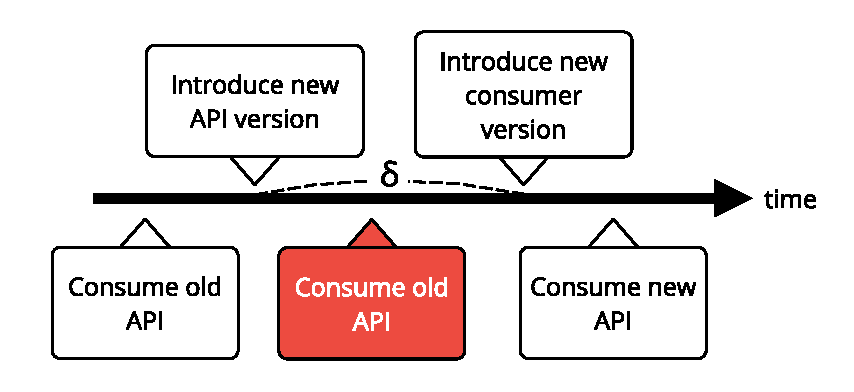
\includegraphics[scale=0.7]{images/figures/api_releases.pdf}
\end{center}
\caption{Introducing new non-backward-compatible \ac{API} versions without being able to direct requests at specific versions.}%
\label{fig:api_releases}
\end{figure}

Figure~\ref{fig:api_releases} shows the process of releasing a new \ac{API} and
consumer version. In this process all consumer requests targeted at the
\ac{API} fail from the point at which the new \ac{API} version is deployed to
the point where the new consumer version is deployed (marked as $\delta$).
However the introduction of backward-compatible changes, like the extension of
a resource schema, can be done without having to expect any downtime
\autocite{MicrosoftAPIdesign2018}.

Regardless of the versioning method discussed further along on this section,
\ac{API} versions generally do not follow the SemVer or CalVer schemas.
Instead, simple integers are used which, in some cases, are prefixed with the
character \texttt{v}.

The first and possibly easiest way to version an \ac{API} is to include the
\ac{API}'s version number in the \ac{URI}. An \ac{API}'s \ac{URI} hence may
look like this: \texttt{https://api.example.net/v1/users/1}. This way, whenever
resources change in a compatibility-breaking form, the \ac{API}'s version
number is incremented. \autocite[Ch. 6]{MasseRESTAPIDesign2011} however argues
that a \ac{URI} based \ac{API} versioning should be avoided. According to
\autocite{MasseRESTAPIDesign2011}, a resource in the context of \ac{REST}
\acp{API} is a \enquote{semantic model, like a thought about a thing}.
A resource only has one identity and a resource's identity
is its full \ac{URI}. Thus a \ac{URI} based version number is part of a
resource's identity. This would imply that different version numbers inside the
\ac{URI} denote that the concept of the resource has multiple version
\autocite[Ch. 6]{MasseRESTAPIDesign2011}. In addition to this,
\autocite{MicrosoftAPIdesign2018} argues that resources that describe the same
data simply should not be able to be addressed using different \acp{URI}.

Instead of including the \ac{API} version number in the resource \ac{URI}, it
is possible to include a custom header in the consumer's request. This way, the
consumer can specify the \ac{API} version independently from the resource by
e.g.\ supplying a header field \texttt{API-Version: v1}
\autocite{MicrosoftAPIdesign2018}.

These are the two most commonly used methods for supplying a version to an
\ac{API}. For the purpose of this thesis, these two are sufficient. If
required, \autocite{MicrosoftAPIdesign2018} outlines two additional methods.
